% Автор разбора: Антон Ахи

\begin{frame}
  \frametitle{Задача <<Огромная парковка>>}
  \begin{center}
    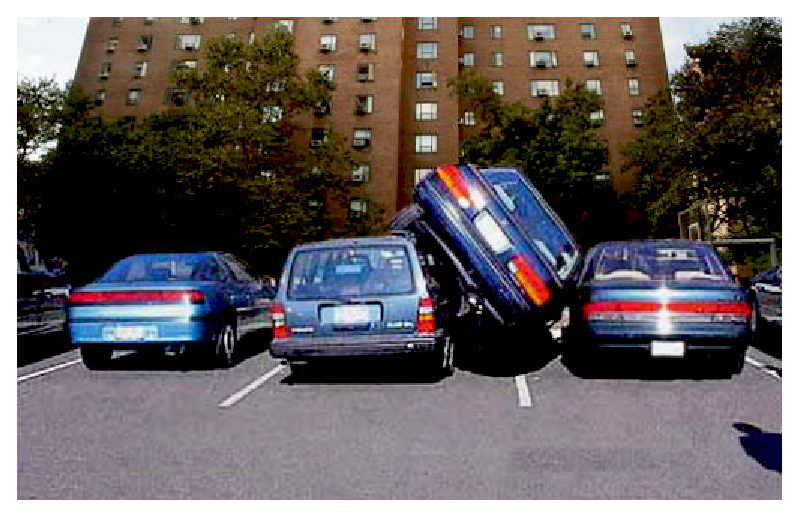
\includegraphics[width=10cm]{parking.eps}
  \end{center}
\end{frame}

\begin{frame}
  \frametitle{Над задачей работали}
  \begin{itemize}
    \item Идея задачи: Георгий Корнеев
    \item Текст условия: Антон Ахи
    \item Тесты, проверяющая программа и др.: Сергей Поромов
    \item Решения: Сергей Мельников, Антон Банных, Нияз Нигматуллин, Сергей Поромов
    \item Текст разбора: Антон Ахи
  \end{itemize}
\end{frame}

\begin{frame}
  \frametitle{Формулировка задачи}
  \begin{itemize}
    \item На огромной парковке много автомобилей и столбов, а также одно свободное место
    \item Хочется вывести один из автомобилей с парковки
    \item Разрешается сдвигать любую машину на соседнее место, если оно свободно
  \end{itemize}
\end{frame}

\begin{frame}
  \frametitle{Идея решения}
  \begin{itemize}
    \item Обход в ширину по состояниям
    \item Состояние --- позиция свободного места и машины, которую хочется вывести
    \item Число состояний $O(n^2 \cdot m^2)$
  \end{itemize}
\end{frame}

\begin{frame}
  \frametitle{Как переходить между состояниями}
  \begin{itemize}
    \item Можно <<переместить>> свободное место на соседнюю позицию, если там не столб 
    \item Если эта позиция была занята автомобилем, который необходимо вывести, то необходимо
    		изменить его позицию
    \item Переход между состояниями совершается за $O(1)$      
  \end{itemize}
\end{frame}

\begin{frame}
  \frametitle{Итого}
  \begin{itemize}
    \item Алгоритм совершает $O(m^2 \cdot n^2)$ операций и требует $O(m^2 \cdot n^2)$ памяти 
    \item Вопросы?
  \end{itemize}
\end{frame}
